% Mineração e sensibilidade de métricas DORA em repositórios open-source
% Laboratório de Experimentação de Software — PUC Minas
%
% Compilação: requer o template oficial da SBC (sbc-template.sty e sbc.bst) nesta pasta.
% Veja artigo/README.md.
\documentclass[12pt]{article}

\usepackage{sbc-template}
\usepackage{graphicx,url}
\usepackage[brazil]{babel}
\usepackage[utf8]{inputenc}
\usepackage{amsmath}   % \text{} nas fórmulas da Seção 2
\usepackage{booktabs}
\usepackage{multirow}

% As figuras são geradas por `python -m analise` e não são editadas à mão.
% As figuras ficam em artigo/figuras/ (Overleaf) ou em resultados/figuras/ (repo).
\graphicspath{{.}{../resultados/}}

\sloppy

\title{Mineração e Sensibilidade de Métricas DORA em Repositórios\\
       Open-Source: a Definição Operacional como Variável do Estudo}

\author{Rafael Faria Franco\inst{1}, Paulo Assis\inst{1}, Vitor Rebula Nogueira\inst{1}}

\address{ICEI --- Pontifícia Universidade Católica de Minas Gerais (PUC Minas)\\
  Belo Horizonte, MG, Brasil
  \email{\{matricula1,matricula2,matricula3\}@sga.pucminas.br}
}

\begin{document}

\maketitle

\begin{resumo}
As métricas DORA (\emph{DevOps Research and Assessment}) consolidaram-se como padrão
industrial de medição de entrega contínua, mas sua aplicação a projetos open-source exige
\emph{proxies} operacionais, porque o GitHub não registra deploys nem falhas em produção.
Este trabalho minera as quatro métricas em 300 repositórios populares que usam GitHub
Actions, na janela de 2025, a partir de 18.389 releases e 20.117 episódios de falha de CI.
A amostra apresenta mediana de 0,46 release por semana, lead time por release de 324,9 h,
\emph{change failure rate} de CI de 0,056 e recuperação de 4,94 h. O achado central não é
nenhum desses valores, e sim a sua dependência da definição adotada: a análise de
sensibilidade mostra que até 31,3\% dos repositórios mudam de categoria DORA entre
combinações ($\kappa$ ponderado de 0,506) e que trocar a \emph{variante da métrica} desloca
a classificação quase quatro vezes mais do que trocar a \emph{unidade de deploy}
(28,3\% contra 7,3\%). Mostra-se ainda que 86,3\% dos repositórios mudam de categoria geral
se uma única métrica avançar um degrau de faixa, o que implica que divergências entre
execuções independentes não constituem, por si, erro de cálculo.
\end{resumo}

\section{Introdução}

As práticas de entrega contínua consolidaram o programa \emph{DevOps Research and
Assessment} (DORA) como a taxonomia padrão de medição de desempenho de entrega
\cite{forsgren2018}. Os quatro construtos --- \emph{deployment frequency}
(frequência de deploy), \emph{lead time for changes} (tempo entre o commit e a entrega),
\emph{change failure rate} (taxa de falha das mudanças) e tempo de recuperação após falha
--- sustentam a tese de que equipes maduras entregam rápido \emph{e} com
estabilidade, rompendo o \emph{trade-off} clássico entre velocidade e confiabilidade
\cite{dora2024}.

A literatura que originou essas faixas apoia-se em telemetria direta de ambientes
produtivos. Avaliar o ecossistema open-source impõe uma barreira metodológica diferente: o
GitHub não registra instantes de entrada em produção nem interrupções de serviço. Estudos
empíricos operam, por isso, com \emph{proxies} --- aproximações indiretas em que a
publicação de uma release assume o papel de deploy e a falha de um \emph{workflow} de
integração contínua assume o papel de falha de entrega.

O uso acrítico desses \emph{proxies} ameaça a validade de construto. Uma biblioteca
publicada mensalmente não faz deploy em produção; quem o faz é quem consome a dependência.
Da mesma forma, uma execução de CI que falha em um \emph{pull request} não representa
necessariamente um defeito que chegou ao usuário. A pergunta que organiza este trabalho é,
portanto, menos "qual é o valor da métrica" e mais: \textbf{o quanto as conclusões empíricas
dependem da definição operacional adotada?}

Registramos, antes de observar os dados, uma hipótese informal por questão de pesquisa,
acompanhada da razão de esperá-la:

\begin{itemize}
  \item \textbf{RQ 01 (frequência de deploy).} \emph{H1:} concentração em \emph{Elite}/\emph{High}, por serem
    projetos de CI maduro e publicação automatizada.
  \item \textbf{RQ 02 (tempo entre o commit e a entrega).} \emph{H2:} as duas variantes produzem valores próximos, por
    medirem o mesmo intervalo por caminhos distintos.
  \item \textbf{RQ 03 (taxa de falha das mudanças).} \emph{H3:} taxa baixa (\emph{Elite}) e variantes concordantes,
    por haver suítes extensas e revisão antes da integração.
  \item \textbf{RQ 04 (tempo de recuperação).} \emph{H4:} mediana inferior a 24 h, porque uma
    \emph{build} quebrada no \emph{default branch} bloqueia todos os contribuidores.
  \item \textbf{RQ 05 (frequência de deploy $\times$ taxa de falha).} \emph{H5:} sem \emph{trade-off} entre velocidade e
    estabilidade, como sustenta o relatório DORA.
  \item \textbf{RQ 06 (fatores estruturais).} \emph{H6:} popularidade associa-se a melhor desempenho,
    por atrair mantenedores e investimento em automação.
  \item \textbf{RQ 07 (análise de sensibilidade).} \emph{H7:} conclusões robustas à definição, por todas
    tentarem capturar o mesmo fenômeno.
  \item \textbf{RQ 08 (taxa de retrabalho).} \emph{H8:} taxa baixa e fortemente correlacionada à taxa de falha
    de entrega, por derivarem da mesma heurística.
\end{itemize}

O restante do artigo organiza-se como segue: a Seção \ref{sec:metodologia} descreve o funil
amostral, as definições operacionais, as combinações da análise de sensibilidade, a
validação manual e a engenharia do \emph{pipeline}; a Seção \ref{sec:resultados} sintetiza
os achados das RQ 01 a 08; a Seção \ref{sec:discussao} confronta as hipóteses com os dados;
a Seção \ref{sec:ameacas} expõe as ameaças à validade; a Seção \ref{sec:replicacao} relata a
replicação cruzada nas duas direções; e a Seção \ref{sec:conclusao} encerra o estudo.

\section{Metodologia}
\label{sec:metodologia}

\subsection{Janela de Observação e Funil de Seleção}

A janela compreende os 12 meses de 1º de janeiro a 31 de dezembro de 2025. Só entram no
cálculo releases publicadas e \emph{workflow runs} criados dentro dela, e apenas no
\emph{default branch} de cada repositório. A mineração é executada por \emph{script}
próprio sobre a API REST do GitHub, sem bibliotecas de acesso à API, e é controlada por um
arquivo de parâmetros.

Para contornar o teto de 1.000 resultados por consulta da API de busca, a coleta de
candidatos foi fatiada em cinco faixas contínuas de estrelas, de \texttt{stars:1000..2000}
até \texttt{stars:>20000}. O funil aplicou os filtros em ordem crescente de custo de API ---
cada um só é consultado se o anterior passou --- até a amostra final de 300 repositórios
(Tabela \ref{tab:funil}).

\begin{table}[ht]
\centering
\caption{Funil de seleção sistemática da amostra.}
\label{tab:funil}
\footnotesize
\begin{tabular}{clrr}
\toprule
\textbf{\#} & \textbf{Etapa} & \textbf{Restantes} & \textbf{Descartes} \\
\midrule
1 & Candidatos recebidos da busca fatiada por estrelas & 1.025 & --- \\
2 & Repositórios únicos, após remoção de duplicatas entre faixas & 1.021 & 4 \\
3 & Com GitHub Actions (\texttt{total\_count} $>$ 0 em \emph{workflows}) & 917 & 103 \\
4 & Com 5 ou mais releases publicadas na janela & 406 & 511 \\
5 & Com 50 ou mais \emph{workflow runs} válidos na janela & 300 & 106 \\
\midrule
6 & \textbf{Amostra final} & \textbf{300} & --- \\
\bottomrule
\end{tabular}
\end{table}

O descarte dominante é o critério de inclusão de releases: 511 repositórios populares e com
CI configurado publicaram menos de cinco releases em doze meses. Um repositório foi perdido
por erro de coleta não recuperável.

\subsection{Definições Operacionais Comuns}

As regras abaixo são idênticas para toda a turma. A \textbf{unidade de deploy} é a release
publicada (\texttt{draft = false}); pré-releases e \emph{tags} entram apenas como variantes na
RQ 07. A \textbf{data de commit} vem de \texttt{commit.author.date}. A \textbf{frequência}
(RQ 01) é a razão entre releases válidas e as 52,1 semanas da janela. No \textbf{lead time}
(RQ 02), os commits de cada release $R$ vêm de \texttt{compare/\{anterior\}...\{R\}}: a
variante (a) é a publicação de $R$ menos o commit mais antigo nela incluído, e a (b) atribui a
cada commit a diferença até a publicação da sua release, com mediana por repositório em ambas.
Na \textbf{taxa de falha das mudanças} (RQ 03), a variante (a) é falhas sobre falhas mais sucessos dos \emph{runs}
considerados --- \texttt{failure}, \texttt{timed\_out} e \texttt{startup\_failure} contam como
falha, enquanto \texttt{cancelled}, \texttt{skipped}, \texttt{neutral},
\texttt{action\_required}, \texttt{stale} e execuções em andamento são ignorados --- e a (b)
marca como falha a release sucedida, em até 7 dias, por uma corretiva da mesma linha
\emph{major.minor}. A \textbf{recuperação} (RQ 04) vai do \texttt{run\_started\_at} da
primeira falha ao \texttt{updated\_at} do primeiro sucesso do \emph{mesmo workflow}. Medições
cujo evento final não ocorre na janela não são descartadas: episódios sem sucesso posterior e
releases dos últimos 7 dias são registrados como \textbf{censurados} e reportados junto das
estatísticas.

Todas as métricas são resumidas por \textbf{mediana e IQR}, nunca por média e
desvio-padrão, porque as distribuições são assimétricas (Figura \ref{fig:violino}).
Correlações usam Spearman ($\rho$), com Pearson ($r$) apenas como contraste; comparações
entre grupos usam Kruskal-Wallis com correção de Holm, $\varepsilon^2$ e Cliff's $\delta$
interpretado por \citeonline{romano2006}; a concordância entre classificações usa $\kappa$
de Cohen ponderado linear, interpretado por \citeonline{landis1977}.

\subsection{Combinações de Definições (C1 a C4)}

A análise de sensibilidade (RQ 07) compara quatro combinações, desenhadas para
\emph{separar} o efeito de trocar a unidade de deploy do de trocar a variante da métrica
(Tabela \ref{tab:combinacoes}). C1 e C4 diferem apenas nas variantes; C2 e C4, apenas na
unidade.

\begin{table}[ht]
\centering
\caption{Combinações de definições operacionais da análise de sensibilidade.}
\label{tab:combinacoes}
\footnotesize
\begin{tabular}{llll}
\toprule
\textbf{Combinação} & \textbf{Unidade de deploy} & \textbf{Lead time} & \textbf{Taxa de falha} \\
\midrule
C1 (referência) & release & (a) por release & (a) de integração contínua \\
C2 & release + pré-release & (b) por commit & (b) de entrega \\
C3 & tag & (b) por commit & (a) de integração contínua \\
C4 & release & (b) por commit & (b) de entrega \\
\bottomrule
\end{tabular}
\end{table}

A C1 usa \emph{estritamente} a variante (a) do lead time: um repositório sem ela fica sem
classificação nessa métrica, em vez de recair sobre a (b). Aceitar esse recuo colocaria
repositórios híbridos C1/C4 dentro da referência e contaminaria exatamente a comparação que
a Tabela \ref{tab:combinacoes} foi desenhada para permitir.

\subsection{Validação Manual e Amostra-Ouro}

Para avaliar a validade de construto dos \emph{proxies}, sorteamos 60 repositórios da
amostra final com semente fixa e documentada, e rotulamos 300 releases (cinco por
repositório) em três dimensões: o tipo do projeto, se as releases representam entregas
reais ao usuário, e se cada release é corretiva. Os rótulos de consenso do grupo estão
versionados no repositório.

O rótulo de entrega real sustenta diretamente a discussão de "release $\neq$ deploy":
\textbf{295 das 300 releases} foram rotuladas como representando entregas reais ao usuário
e 5 ficaram como incertas, sem nenhuma rotulada como "não". Quanto ao tipo, 135 releases
pertencem a aplicações ou serviços, 95 a bibliotecas ou \emph{frameworks} e 70 a
ferramentas de linha de comando; essa classificação alimenta o fator "tipo do projeto" da
RQ 06.

A heurística de release corretiva foi avaliada contra o consenso. A versão v1 --- mudança
apenas de \emph{patch} em relação à anterior da mesma linha ou, fora do SemVer, ao menos
metade das mensagens de commit citando \texttt{fix}, \texttt{hotfix} ou \texttt{revert} ---
obteve precisão de 0,696, \emph{recall} de 0,824 e \textbf{F1 de 0,754}, com 55 falsos
positivos e 27 falsos negativos sobre as 300 releases. Como o F1 superou o limiar de 0,70,
a v1 foi oficializada sem refinamento, e nenhuma versão posterior foi necessária.

\subsection{Engenharia do \emph{Pipeline} e Limites de API}

O \emph{pipeline} é executável por um único comando documentado no README, com o token lido
apenas da variável \texttt{GITHUB\_TOKEN} e nunca versionado. Cada resposta da API é
persistida em disco e um diário de retomada por etapa permite que uma execução interrompida
por \emph{rate limit}, queda de rede ou \texttt{Ctrl+C} continue de onde parou, sem repetir
chamadas. O cliente lê \texttt{X-RateLimit-Remaining} e \texttt{X-RateLimit-Reset} e aguarda
antes de exaurir a cota, repetindo erros 5xx com \emph{backoff} exponencial. A janela de
\emph{workflow runs} é subdividida por mês, com subdivisão adaptativa quando um período se
aproxima do teto de 1.000 resultados, e a comparação entre releases é paginada para
ultrapassar o limite de 250 commits. As funções de cálculo são testadas com \emph{fixtures}
calculadas à mão, incluindo os casos de borda exigidos --- release sem commits novos, falha
nunca recuperada, repositório com uma única release e execuções \texttt{cancelled}; a suíte
tem 729 testes, cobertura de 97,9\% e roda no GitHub Actions do grupo a cada \emph{push}, em
duas versões de Python. Todas as tabelas e figuras deste artigo são geradas por
\texttt{python -m analise} a partir dos CSVs publicados, sem chamar a API, e cada coluna
desses CSVs está documentada no dicionário de dados do repositório.

\section{Resultados}
\label{sec:resultados}

Esta seção apresenta os números sem interpretá-los; a leitura vai para a Seção
\ref{sec:discussao}. Todos os valores são gerados por \texttt{python -m analise} sobre 300
repositórios, 18.389 releases e 20.117 episódios de falha.

\subsection{Estatísticas Descritivas e Classificação DORA (RQ 01 a 04)}

A Tabela \ref{tab:sintese} consolida mediana, quartis, IQR e o nível DORA resultante na
combinação de referência C1. A Figura \ref{fig:violino} mostra a forma das distribuições: as
quatro são fortemente assimétricas, e o lead time (a) varia de 1,2 h a mais de 50.000 h.

\begin{table}[ht]
\centering
\caption{Sumário descritivo das métricas DORA na amostra (combinação C1).}
\label{tab:sintese}
\footnotesize
\begin{tabular}{llrrrrrl}
\toprule
\textbf{RQ} & \textbf{Métrica} & \textbf{n} & \textbf{Mediana} & \textbf{Q1} & \textbf{Q3} &
\textbf{IQR} & \textbf{Nível} \\
\midrule
RQ 01 & Frequência (rel./sem.) & 300 & 0,460 & 0,230 & 1,002 & 0,772 & \emph{Medium} \\
RQ 02 & Lead time (a) release & 300 & 324,9 h & 116,7 h & 996,9 h & 880,2 h & \emph{Medium} \\
RQ 02 & Lead time (b) commit & 300 & 411,8 h & 128,2 h & 1.844,3 h & 1.716,2 h & \emph{Medium} \\
RQ 03 & Taxa de falha (a) de integração contínua & 300 & 5,63\% & 1,33\% & 13,29\% & 11,96\% & \emph{Elite} \\
RQ 03 & Taxa de falha (b) de entrega & 300 & 26,92\% & 10,54\% & 50,00\% & 39,46\% & \emph{High} \\
RQ 04 & Recuperação (horas) & 264 & 4,94 h & 1,75 h & 18,75 h & 17,00 h & \emph{High} \\
\bottomrule
\end{tabular}
\end{table}

\begin{figure}[ht]
\centering
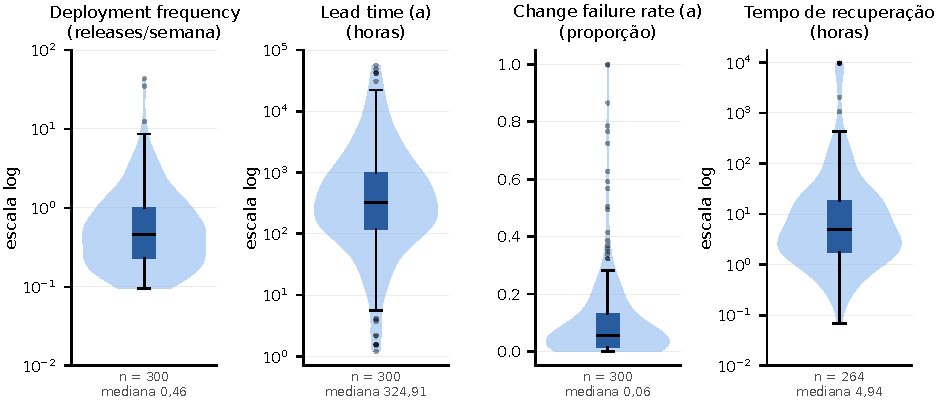
\includegraphics[width=0.85\textwidth]{figuras/artigo_violino_metricas.pdf}
\caption{Distribuição das quatro métricas da C1, com violino para a forma e boxplot interno
para mediana e IQR. Unidades diferentes não compartilham eixo: cada métrica ocupa seu
painel, e três delas estão em escala logarítmica.}
\label{fig:violino}
\end{figure}

A distribuição dos 300 repositórios na classificação geral C1 resultou em \emph{Elite}: 9
(3,0\%), \emph{High}: 110 (36,7\%), \emph{Medium}: 154 (51,3\%) e \emph{Low}: 27 (9,0\%). Por
métrica (Tabela \ref{tab:c1}), chama atenção a concentração da taxa de falha (a): 234 dos 300
repositórios caem em \emph{Elite}.

\begin{table}[ht]
\centering
\caption{Distribuição das categorias DORA por métrica na combinação C1.}
\label{tab:c1}
\footnotesize
\begin{tabular}{lrrrrr}
\toprule
\textbf{Métrica} & \textbf{Elite} & \textbf{High} & \textbf{Medium} & \textbf{Low} &
\textbf{Sem class.} \\
\midrule
Deployment frequency & 6 & 69 & 152 & 73 & 0 \\
Lead time (a) & 25 & 81 & 93 & 101 & 0 \\
Taxa de falha das mudanças (a) & 234 & 47 & 8 & 11 & 0 \\
Tempo de recuperação & 33 & 181 & 33 & 21 & 32 \\
\midrule
\textbf{Classificação geral} & \textbf{9} & \textbf{110} & \textbf{154} & \textbf{27} & \textbf{0} \\
\bottomrule
\end{tabular}
\end{table}

\textbf{Auditoria de integridade e censura.} Nada foi estimado para fechar conta. No lead
time, 3.052 das 18.389 releases (16,6\%) ficaram fora por motivo explícito, sendo 3.026 por
não trazerem commits novos, 23 por não terem release anterior e 3 por erro de
\texttt{compare} (2 deles 404). Na taxa de falha (a) entraram 730.432 \emph{workflow runs} e foram
ignorados 60.959 (7,7\%). Na taxa de falha (b), 246 releases (1,3\%) dos últimos 7 dias ficaram fora do
denominador, restando 18.143 avaliadas, das quais 10.974 falharam. Na RQ 04, dos 20.117
episódios, 19.921 foram recuperados, 196 censurados e 124 com datas contraditórias; 36 dos
300 repositórios (12,0\%) ficam sem mediana por não terem episódio recuperado e consistente.
A proporção censurada por repositório tem mediana 0,0\% e Q3 2,9\%, e tratar cada censurado
como recuperado no fim da observação --- limite inferior do viés --- eleva a mediana de
4,94 h para 5,22 h.

\subsection{Velocidade $\times$ Estabilidade (RQ 05)}

A correlação de Spearman revelou comportamento assimétrico entre os dois \emph{proxies}
(Figura \ref{fig:dispersao}). Com o \emph{proxy} de integração contínua, a associação é desprezível e não
significativa ($\rho = 0{,}071$; $p = 0{,}222$; $n = 300$). Com o \emph{proxy} de entrega, é
moderada e fortemente significativa ($\rho = 0{,}615$; $p = 1{,}2 \times 10^{-32}$).

\begin{figure}[ht]
\centering
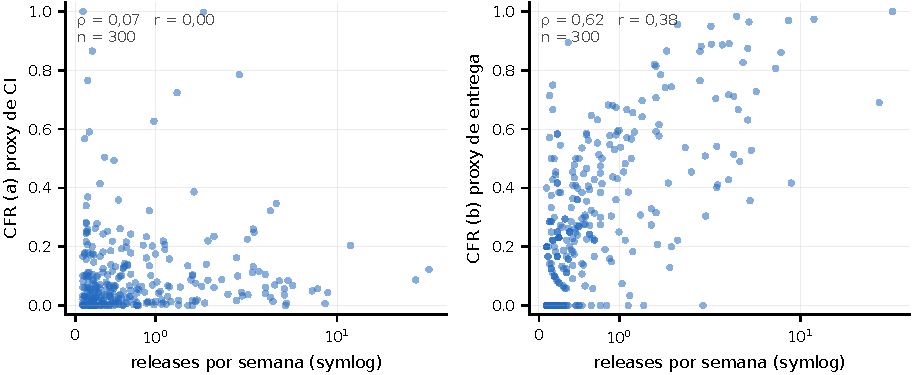
\includegraphics[width=0.85\textwidth]{figuras/artigo_dispersao_df_cfr.pdf}
\caption{Dispersão entre frequência de deploy e \emph{change failure rate} nas duas
variantes, com $\rho$ de Spearman e $r$ de Pearson anotados em cada painel.}
\label{fig:dispersao}
\end{figure}

O diagnóstico da janela de sete dias quantifica o mecanismo por trás do segundo
coeficiente: entre os repositórios do quartil inferior de frequência, o intervalo mediano
entre releases é de 27,9 dias e apenas 25,0\% dos intervalos cabem em sete dias; no quartil
superior, o intervalo mediano é de 1,39 dia e 87,7\% cabem na janela.

A Figura \ref{fig:correlacao} estende a análise a todos os pares de métricas, com Spearman e
Pearson lado a lado. A diferença entre os dois coeficientes é sistemática: em
frequência $\times$ lead time (a), $\rho = -0{,}575$ contra $r = -0{,}066$; em lead
time (a) $\times$ taxa de falha (b),
$-0{,}717$ contra $-0{,}263$.

\begin{figure}[ht]
\centering
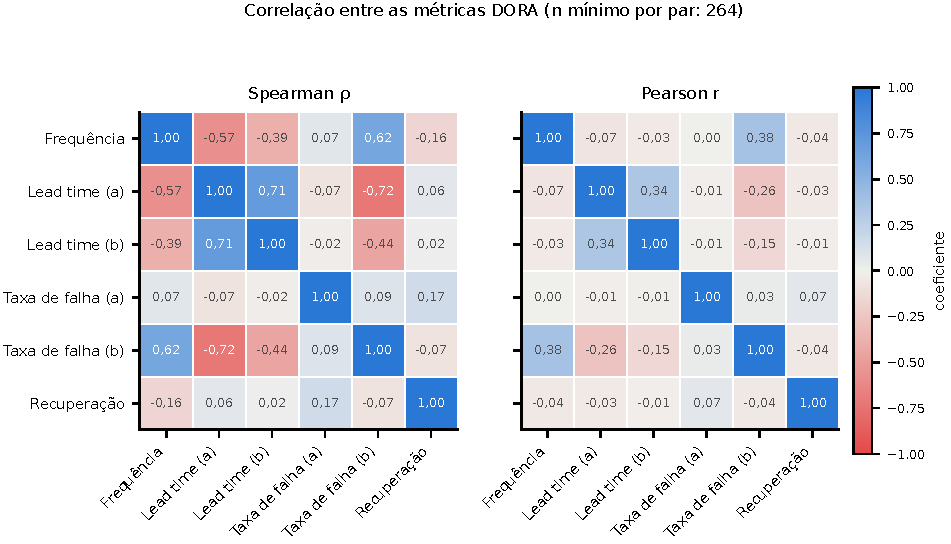
\includegraphics[width=0.85\textwidth]{figuras/artigo_correlacao.pdf}
\caption{Matriz de correlação entre as métricas, com Spearman à esquerda e Pearson à
direita, na mesma escala divergente. O painel de Pearson é sistematicamente mais pálido.}
\label{fig:correlacao}
\end{figure}

\subsection{Fatores Estruturais e Desempenho DORA (RQ 06)}

Após a correção de Holm sobre a família de 16 testes, quatro combinações de fator e métrica
rejeitam a hipótese nula, todas envolvendo linguagem ou número de contribuidores. A
linguagem principal é o fator mais forte, com efeito médio sobre o lead time (a)
($\varepsilon^2 = 0{,}164$; $p_{\text{Holm}} = 9{,}4 \times 10^{-8}$; $n = 299$) e sobre a
frequência ($\varepsilon^2 = 0{,}113$; $p_{\text{Holm}} = 7{,}7 \times 10^{-5}$). O número
de contribuidores segue, com efeito médio no lead time ($\varepsilon^2 = 0{,}100$;
$p_{\text{Holm}} = 1{,}5 \times 10^{-5}$) e pequeno na frequência
($\varepsilon^2 = 0{,}046$; $p_{\text{Holm}} = 0{,}0296$). A popularidade medida em estrelas
\textbf{não} apresenta significância após a correção em nenhuma das quatro métricas: o caso
mais próximo, estrelas contra frequência, passa de $p = 0{,}0070$ bruto para
$p_{\text{Holm}} = 0{,}0556$, e os demais ficam em $p_{\text{Holm}} = 1{,}000$ com
$\varepsilon^2 \leq 0{,}007$. O fator idade não pôde ser testado: a estratificação por
quartis não produziu dois grupos válidos na amostra.

\begin{figure}[ht]
\centering
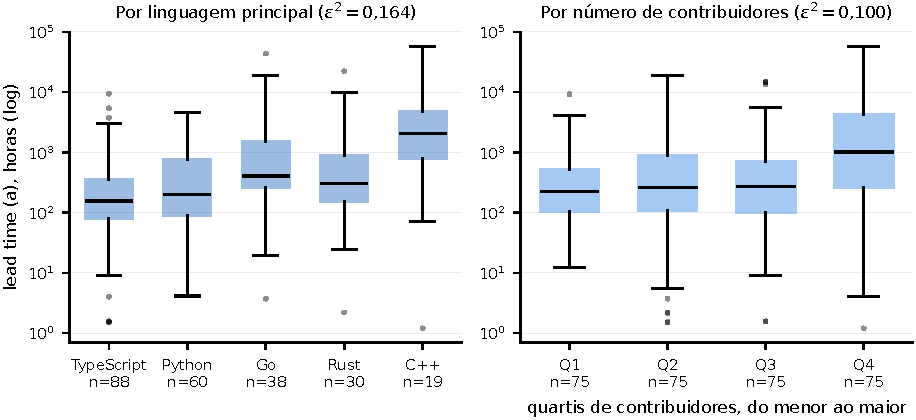
\includegraphics[width=0.85\textwidth]{figuras/artigo_rq06_fatores.pdf}
\caption{Lead time (a) por linguagem principal e por quartil de contribuidores, em escala
logarítmica. As caixas mostram mediana e IQR, e o $n$ de cada grupo está no eixo.}
\label{fig:rq06}
\end{figure}

\subsection{Análise de Sensibilidade e Retrabalho (RQ 07 e RQ 08)}

A Tabela \ref{tab:rq07} apresenta, para cada par de combinações, a proporção de
repositórios que mudam de categoria geral e o $\kappa$ ponderado correspondente.

\begin{table}[ht]
\centering
\caption{Sensibilidade da classificação às definições operacionais ($n = 300$).}
\label{tab:rq07}
\footnotesize
\begin{tabular}{llrrl}
\toprule
\textbf{Par} & \textbf{O que muda} & \textbf{Mudaram} & \textbf{\%} &
\textbf{$\kappa$ pond. linear} \\
\midrule
C1 $\times$ C2 & unidade e ambas as variantes & 94 & 31,3 & 0,506 (moderada) \\
C3 $\times$ C4 & unidade e variante da taxa de falha & 103 & 34,3 & 0,492 (moderada) \\
C2 $\times$ C3 & unidade e variante da taxa de falha & 100 & 33,3 & 0,507 (moderada) \\
C1 $\times$ C4 & \textbf{só as variantes} & 85 & 28,3 & 0,546 (moderada) \\
C1 $\times$ C3 & unidade e variante do lead time & 73 & 24,3 & 0,651 (substancial) \\
C2 $\times$ C4 & \textbf{só a unidade de deploy} & 22 & 7,3 & 0,878 (quase perfeita) \\
\bottomrule
\end{tabular}
\end{table}

Por métrica isolada, o \emph{change failure rate} é o que mais se desloca: entre C1 e C2 ele
muda de faixa em 72,3\% dos repositórios, com $\kappa = -0{,}015$, ou seja, concordância
nula. A mediana da taxa de falha passa de 5,63\% na C1 para 27,45\% na C2, um aumento de 3,88 vezes.
Em contraste, a frequência de deploy entre C1 e C4 --- que compartilham a unidade --- é
idêntica ($\kappa = 1{,}000$).

\begin{figure}[ht]
\centering
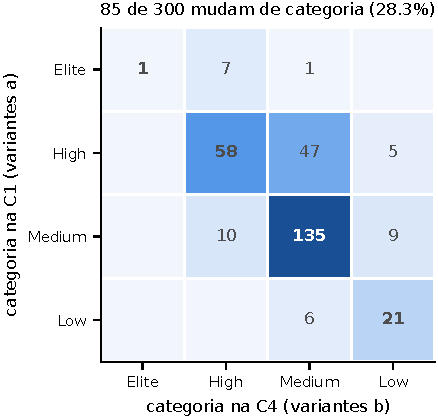
\includegraphics[width=0.52\textwidth]{figuras/artigo_rq07_transicao.pdf}
\caption{Matriz de transição entre a C1 e a C4, que diferem \emph{apenas} nas variantes
das métricas. A diagonal reúne quem permanece na mesma categoria; as 47 transições de
\emph{High} para \emph{Medium} são o deslocamento dominante.}
\label{fig:rq07}
\end{figure}

Para a RQ 08 (bônus), a \emph{deployment rework rate} registrou mediana de 70,0\%
(IQR = 40,6\%; $n = 300$): 12.020 das 18.366 releases avaliadas foram classificadas como
corretivas pela heurística v1, uma taxa agregada de 65,4\%. Sua correlação com a taxa de falha de
entrega é apenas fraca ($\rho = 0{,}359$; $p = 1{,}5 \times 10^{-10}$).

\begin{figure}[ht]
\centering
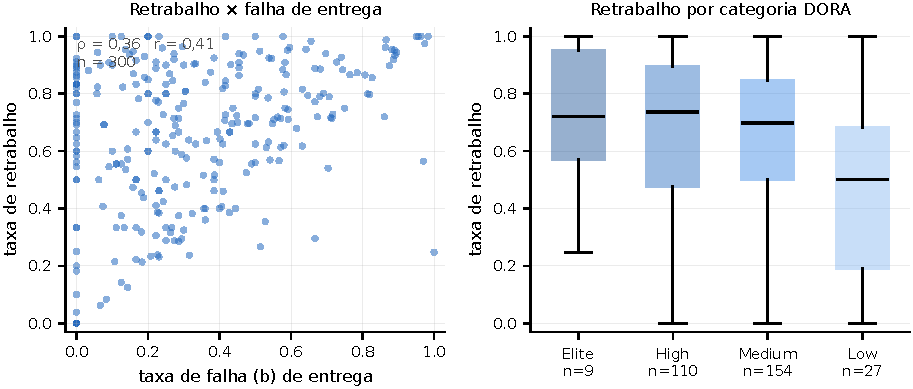
\includegraphics[width=0.85\textwidth]{figuras/artigo_rq08_rework.pdf}
\caption{À esquerda, retrabalho contra taxa de falha (b), com os dois coeficientes. À
direita, retrabalho por categoria geral: a mediana \emph{cai} de 0,72 em \emph{Elite} para
0,50 em \emph{Low}, o inverso do que se esperaria de uma métrica de defeito.}
\label{fig:rq08}
\end{figure}

\subsection{Fragilidade da Classificação nas Fronteiras de Faixa}

Em 259 dos 300 repositórios (86,3\%), mover uma única métrica um degrau de faixa altera a
classificação geral; em 53 (17,7\%) a métrica mais próxima está a 5\% ou menos de um limite,
e em 31 (10,3\%) as duas condições valem simultaneamente. O caso extremo é
\texttt{ultralytics/ultralytics}, a 0,06\% do limite de 24 h do lead time.

\section{Discussão}
\label{sec:discussao}

\subsection{As hipóteses da Introdução contra os resultados}

\begin{table}[ht]
\centering
\caption{As oito hipóteses informais registradas antes da análise, uma por RQ.}
\label{tab:hipoteses}
\footnotesize
\begin{tabular}{p{0.7cm}p{4.4cm}p{5.4cm}l}
\toprule
 & \textbf{Hipótese} & \textbf{Resultado} & \textbf{Veredito} \\
\midrule
H1 & Frequência alta, em \emph{Elite}/\emph{High} &
     Mediana de 0,46 release/semana (\emph{Medium}); 6 \emph{Elite} e 69
     \emph{High} contra 152 \emph{Medium} e 73 \emph{Low} & Refutada \\
H2 & As variantes de lead time são próximas &
     Medianas de 324,9 h e 411,8 h; $\rho = 0{,}71$, mas IQR de 880 h contra 1.716 h &
     Parcial \\
H3 & Taxa de falha baixa e variantes concordantes &
     Taxa de falha (a) mediana 0,056 (\emph{Elite}), mas as variantes discordam em 72,3\% dos
     repositórios, com $\kappa = -0{,}015$ & Parcial \\
H4 & Recuperação abaixo de um dia &
     Mediana de 4,94 h; 181 dos 300 em \emph{High} e 33 em \emph{Elite} &
     Confirmada \\
H5 & Sem \emph{trade-off} velocidade × estabilidade &
     Confirma-se com a variante (a) ($\rho = 0{,}07$); com a (b), $\rho = 0{,}62$ por
     artefato de construção & Parcial \\
H6 & Estrelas associadas a melhor desempenho &
     Nenhuma das quatro métricas se associa a estrelas após Holm; linguagem e
     contribuidores, sim & Refutada \\
H7 & Conclusões robustas à definição &
     Até 31,3\% mudam de categoria; trocar a variante pesa quase 4× mais que trocar a
     unidade & Refutada \\
H8 & Retrabalho baixo e próximo da taxa de falha (b) &
     Mediana de 0,70 (alta) e correlação apenas fraca com a taxa de falha (b)
     ($\rho = 0{,}36$) & Refutada \\
\bottomrule
\end{tabular}
\end{table}

\subsection{Por que as Duas Variantes de Lead Time Divergem (H1 e H2)}

A H1 foi \textbf{refutada}: a mediana de 0,46 release por semana equivale a uma entrega a
cada 15 dias e enquadra a amostra em \emph{Medium}; apenas 6 dos 300 repositórios publicam
diariamente ou mais. Projetos open-source populares operam em regime descontínuo, agrupando
mudanças em lotes mesmo com automação madura.

A H2 foi \textbf{parcialmente confirmada}, e o modo como falha é informativo. As variantes
correlacionam-se fortemente ($\rho = 0{,}71$), mas divergem em dispersão: a (b) tem IQR de
1.716 h contra 880 h da (a). A razão é estrutural --- a (a) é definida pelo commit \emph{mais
antigo} de cada release, a (b) pela mediana de \emph{todos}. Basta um commit antigo esquecido
no intervalo (um \emph{branch} retomado, um \emph{cherry-pick}, um \emph{pull request}
parado) para a (a) subir sem que o ritmo de trabalho mude. Elas respondem a perguntas
distintas: a (a), "quanto tempo cabe dentro de uma entrega"; a (b), "quanto tempo um commit
típico espera para ser entregue".

\subsection{Falha de Pipeline Não é Falha em Produção (H3 e H4)}

A H3 foi \textbf{parcialmente confirmada}: a taxa é baixa pelo \emph{proxy} de integração contínua (5,63\%,
\emph{Elite}, com 234 dos 300 nessa faixa), mas a previsão de concordância entre as variantes
erra por larga margem --- elas discordam de faixa em 72,3\% dos repositórios, com
$\kappa = -0{,}015$. A diferença não é de calibração, é de objeto: uma execução de CI
vermelha é, quase sempre, um teste quebrado em um \emph{pull request} --- barata, detectada
antes da entrega e frequentemente a prova de que o CI funciona. Uma release seguida de
corretiva em sete dias é um defeito que atravessou o pipeline e chegou ao usuário. O
\emph{proxy} de CI mede a barreira; o de entrega mede o que passou por ela. Comparar qualquer
um deles diretamente com as faixas do relatório DORA, que tratam de produção, induz a erro.
A H4, por sua vez, foi \textbf{confirmada}: a recuperação mediana de 4,94 h fica bem abaixo
das 24 h previstas, com 181 repositórios em \emph{High}.

\subsection{O \emph{Trade-off} que é Artefato de Construção (H5)}

Com o \emph{proxy} de integração contínua, a ausência de \emph{trade-off} se confirma ($\rho = 0{,}07$, não
significativo). Com o de entrega, a correlação é positiva e moderada ($\rho = 0{,}62$), o que
contradiria o DORA e sugeriria que entregar mais causa mais falhas. O diagnóstico da janela
de sete dias mostra que a leitura é um \textbf{artefato da própria métrica}: no quartil
superior de frequência, 87,7\% dos intervalos entre releases cabem em sete dias, contra
25,0\% no quartil inferior. Quem publica a cada 1,4 dia quase sempre tem uma release seguinte
dentro da janela de observação da heurística, e portanto muito mais chance de ser marcado
como falha. O numerador e o denominador compartilham a mesma causa --- a cadência --- e o
coeficiente mede cadência disfarçada de estabilidade. Correlação não implica causalidade;
aqui sequer há correlação legítima a interpretar.

\subsection{O Peso da Definição Operacional (H6, H7 e H8)}

A H6 foi \textbf{refutada} no que previa: estrelas não se associam a nenhuma métrica após
Holm, operando como indicador de reputação desacoplado do fluxo de engenharia. Sobrevivem
linguagem e número de contribuidores, ambos com efeito médio. Vale separar significância de
relevância: com $n = 300$, efeitos pequenos alcançam significância sem significar muito.

A H7 foi \textbf{refutada}, e o desenho das combinações permite dizer \emph{como}. Entre C2 e
C4, que diferem apenas na unidade de deploy, 7,3\% mudam de categoria
($\kappa = 0{,}878$); entre C1 e C4, que diferem apenas nas variantes, 28,3\%
($\kappa = 0{,}546$). Ou seja, \textbf{trocar a variante da métrica desloca a classificação
quase quatro vezes mais do que trocar a unidade de deploy}. A discussão sobre se \emph{tag} ou
release conta como deploy importa menos do que a escolha entre a taxa de falha de integração contínua e a de entrega.

A H8 foi \textbf{refutada} nas duas partes: o retrabalho não é baixo (mediana de 70,0\%) e sua
correlação com a taxa de falha de entrega é apenas fraca ($\rho = 0{,}36$), embora ambos derivem da
mesma heurística. A diferença está na janela: o retrabalho conta toda release corretiva do
período, enquanto a taxa de falha (b) só conta as que \emph{seguem} outra release em até sete dias ---
repositórios que corrigem com calma produzem retrabalho alto e taxa de falha (b) baixa.

Soma-se um achado não previsto: 86,3\% dos repositórios mudam de categoria se uma única
métrica avançar um degrau (Seção \ref{sec:resultados}). A classificação em faixas discretiza
medidas contínuas sem sinalizar quem está na fronteira --- resultado que nasceu de uma
divergência da replicação cruzada (Seção \ref{sec:replicacao}).

\section{Ameaças à Validade}
\label{sec:ameacas}

A estrutura desta seção segue a taxonomia usual de ameaças em engenharia de software
experimental \cite{wohlin2012}. Cada ameaça é apoiada em uma evidência do próprio estudo e
acompanhada da mitigação adotada, ou da razão de não ter sido possível mitigá-la.

\textbf{Validade de Construto.} A equivalência entre release e deploy, e entre
\emph{workflow run} vermelho e falha de entrega, é uma aproximação inerente ao uso de
\emph{proxies}. A amostra-ouro mitiga parcialmente a primeira: 295 das 300 releases
rotuladas representam entregas reais ao usuário, 5 ficaram incertas e nenhuma foi rotulada
como "não" --- a suposição se sustenta nesta amostra. Ela permanece, porém, para as 95
releases de bibliotecas e \emph{frameworks}, em que publicar no registro não implica que
alguém atualizou a dependência. A segunda equivalência é o objeto da Seção
\ref{sec:discussao} e não foi mitigada, e sim \emph{medida}: as duas variantes da taxa de falha
discordam em 72,3\% dos repositórios. A heurística corretiva que sustenta a taxa de falha (b) tem
F1 de 0,754, com 55 falsos positivos e 27 falsos negativos, e superdetecta corretivas ---
marca 65,4\% das releases contra 51\% na rotulagem manual. Além disso,
\texttt{commit.author.date} é vulnerável a \emph{rebase} e \emph{squash merge}, que reescrevem
a data e distorcem o lead time sem relação com o esforço real; mitigamos apenas
contabilizando datas ausentes em vez de estimá-las, e mantendo valores negativos visíveis em
vez de descartá-los. Por fim, há uma ameaça ao próprio instrumento de validação: o consenso
da amostra-ouro foi consolidado em um arquivo único do grupo, e as planilhas individuais dos
três avaliadores não estão versionadas, o que impede recalcular o $\kappa$ de Fleiss e,
portanto, aferir a confiabilidade da rotulagem que sustenta o F1 relatado.

\textbf{Validade Interna.} O principal confundidor identificado é a própria cadência: um
repositório que publica com frequência tem mais oportunidades de ter uma release corretiva
dentro de sete dias, o que infla a taxa de falha (b) independentemente da qualidade. Esse mecanismo
foi quantificado (87,7\% contra 25,0\% dos intervalos dentro da janela) e é reportado junto
do coeficiente, não omitido. Releases publicadas por robôs de automação ---
\emph{release-please}, \emph{semantic-release}, Dependabot --- entram como qualquer outra e
inflam a frequência de projetos que automatizaram a publicação; essa ameaça não foi mitigada,
pois não distinguimos autor humano de robô. Execuções agendadas são excluídas pelo filtro de
evento \texttt{push}, mas execuções com matriz de combinações contam como um único
\emph{run}. O truncamento no fim da janela foi tratado por censura explícita, e não por
descarte, em ambos os pontos em que ocorre: 196 episódios de recuperação (0,97\%) e 246
releases da taxa de falha (b) (1,3\%).

\textbf{Validade Externa.} A amostra é deliberadamente estreita: repositórios públicos com
pelo menos 1.001 estrelas, que usam GitHub Actions, observados em uma única janela anual. O
funil dimensiona o recorte: 511 dos 1.021 candidatos avaliados caíram por publicar menos de
cinco releases em doze meses, e outros 103 por não usarem Actions. Os achados descrevem,
portanto, projetos populares, ativos e automatizados --- não o GitHub como um todo, e muito
menos desenvolvimento corporativo, onde o DORA foi formulado e onde "deploy" tem acesso a
dados de produção que aqui não existem. Pipelines em GitLab CI ou Jenkins estão fora do
alcance do instrumento. A janela única impede ainda qualquer afirmação de tendência: 2025 é
um retrato, não uma série temporal.

\textbf{Validade de Conclusão.} A família principal da RQ 06 executa 16 testes, e a correção
de Holm foi aplicada sobre ela; o efeito é observável --- estrelas contra frequência tem
$p = 0{,}0070$ bruto e $p = 0{,}0556$ corrigido, deixando de ser significativo. Todos os
testes são não paramétricos, o que protege as deduções contra a assimetria documentada na
Figura \ref{fig:violino}, e todos os tamanhos de efeito são reportados junto dos $p$-valores.
A análise exploratória por tipo de projeto apoia-se em 60 repositórios distribuídos em três
tipos, e está declarada como exploratória por isso. A mediana de recuperação usa apenas
episódios recuperados e, por construção, subestima o tempo real, já que os episódios mais
longos são justamente os que não terminam na janela; publicamos o limite inferior que trata
cada censurado como recuperado no fim da observação (5,22 h contra 4,94 h) para dimensionar
esse viés. O $n$ difere entre métricas (264 na recuperação contra 300 nas demais), o que
impede comparações diretas de dispersão entre elas. Por fim, as faixas DORA produzem muitos
empates de fronteira: 86,3\% dos repositórios estão a um degrau de outra categoria, de modo
que comparações de categoria entre estudos precisam reportar essa proximidade, sob pena de
atribuir a erro de cálculo o que é efeito da discretização.

\section{Replicação Cruzada}
\label{sec:replicacao}

A replicação ocorreu nas duas direções sobre uma subamostra determinística de 30
repositórios, sorteada com semente fixa e documentada, seguindo apenas o \texttt{README}
publicado de cada lado.

\subsection{Como Replicadores}

Executamos o \emph{pipeline} do grupo sorteado no commit \texttt{73b739f}, em macOS 27.0.1
(arm64) com Python 3.14.0, em ambiente virtual novo e sem cache. A subamostra saiu do
conjunto ordenado e deduplicado dos 300 repositórios do dataset original deles, com o
\emph{hash} SHA-256 do CSV de origem registrado junto da lista, de modo que o sorteio é
refazível por qualquer pessoa.

\textbf{O estudo foi executável}, com uma ressalva de escopo. Clone, instalação e estimativa
de consumo de API somaram menos de dois minutos sem atrito. A execução completa levou
\textbf{42 min 20 s}, dos quais 91\% foi espera da API, consumindo cerca de 1.676 requisições
--- aproximadamente 2,5 vezes a projeção linear da própria estimativa do \emph{pipeline}.
Todos os artefatos prometidos foram produzidos e a suíte deles passou integralmente (159
testes, 77\% de cobertura). A ressalva: \textbf{não existe forma, documentada ou não, de
executar aquele \emph{pipeline} sobre um conjunto dado de repositórios} --- a seleção sempre
refaz a busca por faixas de estrelas, que depende da contagem de estrelas no instante da
execução. Foi preciso ler o código-fonte e escrever à mão o CSV intermediário que as etapas
seguintes consomem, isto é, sair do \texttt{README}. Seguindo estritamente a documentação, a
replicação cruzada como o estudo a define não é executável naquele \emph{pipeline}.

A reprodução dos valores foi praticamente exata: diferença relativa mediana de
\textbf{0,0\% nas sete métricas}, com concordância de categoria de 100\% em frequência, lead
time e taxa de falha, e de 91,3\% na recuperação ($\kappa$ ponderado de 0,907). As divergências
concentram-se em repositórios com poucos episódios, em que um episódio a mais desloca a
mediana --- o maior desvio relativo chega a 945\% nesse cenário. Abrimos quatro Issues no
repositório do grupo autor: uma de execução e documentação (ausência de parâmetro para a
subamostra) e três de documentação (links apontando para o disco local de um autor,
instalação sem ambiente virtual e contagem de colunas desatualizada).

\subsection{Como Autores}

Recebemos três Issues, todas procedentes, todas corrigidas antes do prazo e todas registradas
no GitHub Projects do grupo. A primeira relatava falha do comando de análise em clone limpo,
porque os CSVs não estavam versionados na \emph{branch} principal --- existiam apenas em uma
\emph{branch} seis commits à frente, nunca integrada; publicamos os três CSVs e a análise
passou a rodar de clone limpo, sem token. A segunda apontava a ausência de parâmetro para
executar sobre a subamostra, exatamente a lacuna que encontramos no \emph{pipeline} deles;
acrescentamos uma opção que recebe a lista e substitui a busca, preservando os critérios de
inclusão. A terceira relatava que um repositório mudara de categoria entre o dataset
publicado e a reexecução: a investigação mostrou que \textbf{não havia erro de cálculo em
nenhum dos lados} --- o repositório está 1,87 h acima do limite de 168 h da recuperação
(1,10\% do valor) e, sendo a categoria geral a mediana das quatro notas arredondada para
baixo, mover uma métrica um degrau basta para alterá-la. Essa Issue originou a análise de
fragilidade de fronteira e a ameaça à validade de conclusão correspondente.

Além das três correções, reproduzir a comparação revelou um defeito que \emph{nenhuma} Issue
apontara: o módulo de análise esperava nomes de coluna que o \emph{pipeline} não escreve e,
como coluna ausente é valor ausente por contrato, lia o CSV real \textbf{sem erro algum e
devolvia estatísticas vazias}. A falha ruidosa encobria uma silenciosa --- o argumento mais
concreto que este trabalho produziu em favor da replicação cruzada.

\section{Conclusão}
\label{sec:conclusao}

Mineramos as quatro métricas DORA em 300 repositórios open-source populares que usam GitHub
Actions, ao longo da janela anual de 2025. A amostra revelou desenvolvimento organizado em
ciclos discretos --- mediana de 0,46 release por semana e lead time por release de 324,9 h
(13,5 dias) --- desafiando a premissa de entrega contínua diária herdada do contexto
corporativo; a maior parte concentra-se em \emph{Medium} (154) e \emph{High} (110), com apenas
9 em \emph{Elite}. A estabilidade percebida varia drasticamente conforme a lente: o
\emph{proxy} de CI sugere maturidade \emph{Elite} (5,63\%), o de entrega indica correção
frequente (26,92\%), e os dois discordam de faixa em 72,3\% dos repositórios.

O achado central não é nenhum desses valores, e sim a sua dependência de escolhas que o
método não torna visíveis. Até 31,3\% dos repositórios migram de categoria entre combinações
e --- graças ao desenho que separa os dois efeitos --- trocar a \textbf{variante da métrica}
desloca a classificação quase quatro vezes mais do que trocar a \textbf{unidade de deploy}
(28,3\% contra 7,3\%). Somado a isso, 86,3\% mudam de categoria se uma única métrica avançar um
degrau, porque as faixas discretizam medidas contínuas sem sinalizar quem está na fronteira.

Decorrem daí três consequências práticas: relatar uma classificação DORA sem explicitar as
definições adotadas não é informativo; a taxa de falha calculada sobre falhas de integração contínua não é comparável às
faixas do relatório DORA, que tratam de produção; e comparações de categoria entre estudos ou
execuções precisam reportar quantos repositórios estavam próximos de um limite, sob pena de
atribuir a erro de cálculo o que é efeito da discretização --- lição que a replicação cruzada
nos impôs na prática.

Como trabalhos futuros, propõem-se validar a heurística corretiva em uma segunda amostra
rotulada, independente daquela em que foi calibrada; estender a observação para além de uma
janela anual, permitindo falar de tendência; e substituir as faixas discretas por uma medida
contínua de desempenho, que não reproduza a fragilidade de fronteira documentada aqui.

\vspace{0.2cm}
\noindent\textbf{Disponibilidade.} Código, dados, dicionário de dados e todas as tabelas e
figuras deste artigo estão em
\url{https://github.com/Paulooassis/Laboratorio-03-medicao-de-software}, reexecutáveis com
\texttt{python -m analise}. O acompanhamento de Issues e sprints está em
\url{https://github.com/Paulooassis/Laboratorio-03-medicao-de-software/projects}.

% A bibliografia acompanha a conclusão: é a última seção do artigo.

\begin{thebibliography}{}

\bibitem[DORA 2024]{dora2024}
DORA (2024).
\newblock {\em DORA's software delivery metrics: the four keys}.
\newblock DevOps Research and Assessment. Disponível em:
  \url{https://dora.dev/guides/dora-metrics-four-keys/}. Acesso em: out. 2026.

\bibitem[Forsgren et al. 2018]{forsgren2018}
Forsgren, N., Humble, J., and Kim, G. (2018).
\newblock {\em Accelerate: The Science of Lean Software and DevOps: Building and
  Scaling High Performing Technology Organizations}.
\newblock IT Revolution Press, Portland, OR.

\bibitem[Landis and Koch 1977]{landis1977}
Landis, J.~R. and Koch, G.~G. (1977).
\newblock The measurement of observer agreement for categorical data.
\newblock {\em Biometrics}, 33(1):159--174.

\bibitem[Romano et al. 2006]{romano2006}
Romano, J., Kromrey, J.~D., Coraggio, J., and Skowronek, J. (2006).
\newblock Appropriate statistics for ordinal level data: Should we really be using
  t-test and Cohen's d for evaluating group differences on the NSSE and other surveys?
\newblock In {\em Annual Meeting of the Florida Association for Institutional
  Research}, pages 1--33.

\bibitem[Wohlin et al. 2012]{wohlin2012}
Wohlin, C., Runeson, P., H{\"o}st, M., Ohlsson, M.~C., Regnell, B., and Wessl{\'e}n,
  A. (2012).
\newblock {\em Experimentation in Software Engineering}.
\newblock Springer, Berlin.

\end{thebibliography}

\end{document}
